\documentclass{beamer}
\usepackage[czech]{babel}
\usepackage[utf8]{inputenc}
%\usepackage[T1]{fontenc}
\usepackage{times}
\usepackage{graphicx}
\usepackage{multirow}
\usepackage{amssymb}

\providecommand{\uv}[1]{\quotedblbase #1\textquotedblleft}

\mode<presentation> {
	\usetheme{Luebeck}
	\setbeamercovered{transparent}
}



\title[\textbf{ZAČÍNÁME S GEOCACHINGEM}]{\huge \textbf{Začínáme s\\GEOCACHINGEM}\\\emph{v deseti krocích}}
\author{V.~Martinka\\ \emph{(xmarti76)}}

\institute{\textsc{Vysoké učení technické v~Brně\\Fakulta informačních technologií}}

\begin{document}
	
	\begin{frame}
		\titlepage
	\end{frame}
	
	\section{Něco málo úvodem}
	\subsection{Našich deset kroků}
	\begin{frame}{Našich deset kroků:}
		%\tableofcontents%[pausesections]
		\begin{enumerate}
			\item Co je geocaching?
			\item Co potřebujeme do začátku?
			\item Vybíráme vhodnou keš
			\item Pozor na různé typy keší
			\item Co je co, aneb čteme listingy
			\item Chováme se nenápadně
			\item Našli jsme, co teď?
			\item Logujeme nález na internetu
			\item A hledáme další\dots
			\item Když něco nevíte
		\end{enumerate}
	\end{frame}
	

	\subsection{Co je geocaching?}
	\begin{frame}{Co je geocaching?}
		\begin{itemize}
			\item Celosvětová hra, která vznikla v roce 2000 v \emph{USA}
			\item Princip hry spočívá v hledání různých skrýší - pokladů nazývaných geocache (zkráceně cache) či česky keš
			\item Ty jsou téměř všude:
				\begin{itemize}
					\item Na vesmírné stanici ISS,
					\item dně oceánu,
					\item ale i za rohem fakulty
				\end{itemize}
			\item A mohou nabývat různých tvarů i velikostí...
		\end{itemize}
%		\begin{figure}[hb]
%			\centering
%			\includegraphics[height=1em]{obr/sizes.jpg}
%			%\caption{Ukázka různých skrýší}
%		\end{figure}
	\end{frame}

	\subsection{Co potřebujeme do začátku?}
	\begin{frame}{Co potřebujeme do začátku?}
		\begin{itemize}
			\item Zařízení s GPS\\
			\begin{table}[ht]
				\catcode`\-=12
				\tiny
				\begin{tabular}[t]{|l|l|l|l|}
					\hline
					                                    & \textbf{Smartphone}                & \textbf{Turistická GPS}        & \textbf{Jiné}\\
					\hline
					\multirow{2}{*}{\textbf{\small +}}  & Má ho téměř každý                  & Delší výdrž na baterie         & Autonavigace,\\
					                                    & Nabízí spoustu doprovodných funkcí & Odolná vůči vodě, pádům, \dots & mapy, buzola,\\
					                                    &                                    &                                & fotografická paměť,\\
					\multirow{2}{*}{\textbf{\small --}} & Horší výdrž na baterii             & Menší počet funkcí             & štěstí, \dots\\
					                                    & Náchylnější na poškození           & Vyšší pořizovací cena          & \\
					\hline
				\end{tabular}
				\normalsize
			\end{table}
			\item Registraci na \url{www.geocaching.com} -- je nutné si vytvořit nějakou vlastní přezdívku $\rightarrow$ \emph{nick}
			\item A to je vše!
		\end{itemize}
	\end{frame}	
	
	\section{Začínáme zjišťováním informací}
	\subsection{Vybíráme vhodnou keš}
	\begin{frame}{Vybíráme vhodnou keš}
		\begin{itemize}
			\item Nejlépe v mapě \texttt{\url{www.geocaching.com} $\rightarrow$ Play \\$\rightarrow$ View Geocache Map}
			\item nebo pomoci vyhledávaní přímo na \url{www.geocaching.com}, popř. v \texttt{Play $\rightarrow$ Find a Geocache} pomocí různých kritérií \emph{(název, oblast, přezdívka autora, apod.)}
			\item Po otevření se dostanete na tzv. listing, tedy souhrn informací o konkrétní schránce
		\end{itemize}	
	\end{frame}
	
	\subsection{Pozor na různé typy keší}
	\begin{frame}{Pozor na různé typy keší}
		\begin{itemize}
			\item \textbf{Tradiční keš} -- najdete ji přímo na uvedených souřadnicích \\
			            \hspace{5.72em} -- nečeká na vás tady žádná záludnost
			\item \textbf{Multi keš}            -- Musíte projít nějakou trasu, během\\
			      \textbf{letterbox}\hspace{0.95em} níž postupně získáte indície,  z kterých \\
			                        \hspace{5.15em} posléze vypočtete souřadnice finální schránky
			\item \textbf{Mystery} -- Budete muset nějakým autorem určeným \\
			           \hspace{4.7em} způsobem získat finální souřadnice \\
			        \hspace{3.8em} -- např. vyluštit doma nějakou šifru nebo i venku \\
			        \hspace{3.8em} -- či jít podle azimutu, zkrátka může jít o cokoli \dots
			\item \textbf{Ostatní} -- Další typy se tak často nevyskytují \\
			       \hspace{3.45em} -- Pro začátečníka spíše nevhodné
		\end{itemize}
	\end{frame}
	
	\subsection{Co je co, aneb čteme listingy}
	\begin{frame}{Co je co, aneb čteme listingy}
		\textbf{Hlavička listingu}
		\begin{itemize}
			\item Obtížnost a terén se hodnotí na stupnici 1 -- 5 $\bigstar$
			\item \emph{Pozor na keše se 4.5 a 5 hvězdičkami!}
		\end{itemize}
		\begin{figure}[hb]
			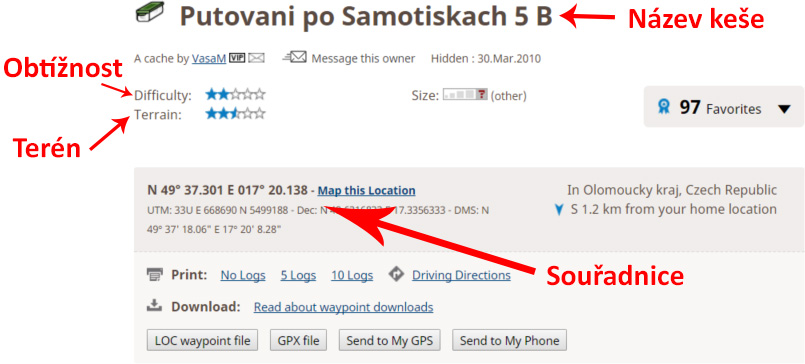
\includegraphics[height=10em]{obr/hlavicka_kese.jpg}
		\end{figure}
	\end{frame}
	
	\begin{frame}{Co je co, aneb čteme listingy}
		\begin{itemize}
			\item Každá keš má dále svůj unikátní \emph{GC-kód}, který slouží pro její jasnou identifikaci
			\item Zpravidla má atributy -- informace doplňující symboly
			\item Obsahuje taktéž tzv. logy, tedy zprávy od dalších hráčů (např. o tom, kdy keš našli, či třeba nenašli)
			\item Samozřejmě popis místa, osobnosti či události, ke které se keš vztahuje, stejně tak i nějaké informace přímo o schránce
			\item a ještě další informace, viz třeba \url{http://wiki.geocaching.cz/wiki/Listing}
		\end{itemize}

	\end{frame}	
	
	\section{Jdeme do terénu}
	\subsection{Chováme se nenápadně}
	\begin{frame}{Chováme se nenápadně}
		\begin{itemize}
			\item Nejlepší je začít tím, že si přečtete listing
			\item Poté je nutné dojít na samotné místo s keší
			\item Může se hodit si přečíst \emph{hint} -- nápověda o autora umístěná na konci listingu
			\item Při hledání se chovejte nenápadně, ideálně tak, aby si vás nikdo nevšímal, cože tam vlastně děláte\dots
			\item Je nutné počítat i s odchylkou systému GPS -- typicky 3~m
			\item Nezapomeňte, že keše mají různou velikost -- podle toho je nutné přizpůsobit okruh hledání (\emph{large} keš nebudu hledat pod okapem, zatímco \emph{micro} nejspíše ano).
		\end{itemize}
	\end{frame}
	

	
	\subsection{Našli jsme ji, co teď?}
	\begin{frame}{Našli jsme, co teď?}
		\textbf{Výborně!}
		\begin{itemize}
			\item Nyní se zapište do deníčku -- \emph{logbooku} vaším nickem, dopište datum (ideálně i čas)
			\item Můžete připojit i nějakou vaši poznámku, popř. poděkování za keš
			\item Ve větších schránkách můžete najít i nějaké drobnosti na výměnu
			\item Zde platí pravidlo, že za cokoli, co si odnesete, máte vložit něco na oplátku a to stejné nebo vyšší hodnoty
			\item \textbf{Pozor}, to se netýká tužky, logbooku, strouhátka a dalších pro keš potřebných věcí
			\item Nakonec nezapomeňte vrátit keš přesně tak, jak byla
		\end{itemize}
	\end{frame}
	
	\section{Zase zpátky k PC}
	\subsection{Logujeme nález na internetu}
	\begin{frame}{Logujeme nález na internetu}
		\begin{itemize}
			\item Po celém dni hledání na vás opět čeká počítač a na ně stránky \url{www.geocaching.com}
			\item Je nutné \emph{zalogovat} všechny keše, které jste našli (ale případně i nenašli)
			\item K tomu slouží odkaz \texttt{Log your visit}, který najdete nahoře v listingu ale i třeba v mapě po rozkliknutí keše, nebo přímo v aplikaci na vašem telefonu
			\item Vyplňte zde datum a typ logu (pro nález slouží \emph{Found it})
			\item Poté napište nějakou krátkou zprávu, kde můžete zmínit zážitky při lovu, poznámky ke keši apod. Nezapomeňte, že to uvidí každý, takže neprozrazujte řešení či překvapení
			\item Na závěr se sluší poděkovat autorovi za keš
		\end{itemize}
	\end{frame}
	
	\subsection{A hledáme další\dots}
	\begin{frame}{A hledáme další\dots}
		\begin{itemize}
			\item Tak a váš první \uv{lov} máte za sebou
			\item Nyní se můžete podívat na další keše, můžete zkusit třeba nějakou mystery keš
			\item Jistě bude vhodné zajít i na nějaký event -- setkání hráčů geocachingu s různým programem, ten zjistíte v listingu
			\item Časem třeba založíte i nějakou svoji keš, ale doporučuji chvíli počkat a nasbírat nějaké zkušenosti
		\end{itemize}
	\end{frame}
	
	\section{A co dál?}
	\subsection{Když něco nevíte}
	\begin{frame}{Když něco nevíte}
		\begin{itemize}
			\item Tato prezentace byla příliš krátká, aby se do ní všechno vlezlo\dots
			\item Na internetu můžete najít spoustu článků vysvětlující geocaching
			\item Nebo se zkuste podívat na \emph{GeoWiki} \url{http://wiki.geocaching.cz}
			\item Pokud vám stále nebude něco jasné, můžete napsat na fórum \url{www.geocaching.cz}
			\item Nebo zajít na nějaký event, tam se určitě najde někdo, kdo vám to vysvětlí nebo třeba s vámi zajde i na nějakou tu keš
		\end{itemize}
	\end{frame}
	
	\begin{frame}
		\centering
		\Huge Děkuji za pozornost
	\end{frame}

\end{document}